
\section{Aufbau}
\label{sec:Aufbau}

\begin{wrapfigure}[24]{r}{7cm}
\vspace{-0.5cm}
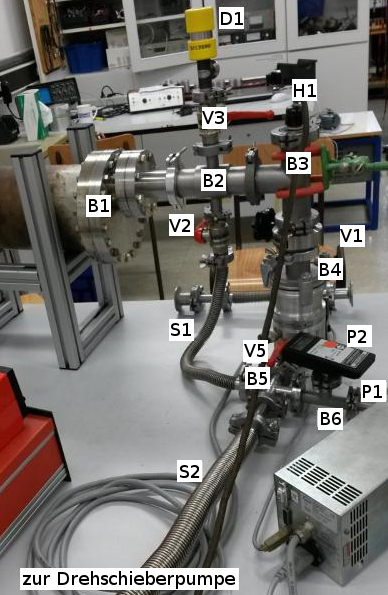
\includegraphics[scale=0.5]{content/images/Aufbau2.jpg}
\caption{Aufbau zum Experiment Vakuumphysik \cite{V70}.}
\label{fig:Aufbau}
\end{wrapfigure}

Der Versuch wird wie in Abbildung \ref{fig:Aufbau} aufgebaut. Am Rezipient (B1) wird über ein Kreuzstück (B2) ein Nadelventil (D1) für die Leckratenmessung der Drehschieberpumpe und alle Messungen der Turbomolekularpumpe angebracht. Über ein Kugelventil (V3) kann dieses komplett geschlossen werden. Über ein T-Stück wird ein Kaltkathoden-Vakuummeter angeschlossen, welches in der Abbildung nicht zu sehen ist. Über ein weiteres T-Stück (B3) mit eingebautem Heizkathoden-Vakuummeter (H1) und ein Klappenventil (V1) wird der Rezipient mit der Turbopumpe verbunden. Mit einem Kugelventil (V2) wird der Tank außerdem über die Schläuche (S1) und (S2) mit der Drehschieberpumpe verbunden, die ebenfalls zur Erzeugung des Vorvakuums der Turbopumpe verwendet wird. Mit dem Kugelventil (V5) kann dies geregelt werden. Über ein kleines Kreuzstück (B5) und ein T-Stück (B6) ist ein analoges und ein digitales Pirani-Vakuummeter (P1 und P2) angeschlossen. Letzteres war bei dieser Durchführung des Versuchs defekt.